\chapter{Nervous system anatomy and physiology}


\begin{description}
    \item[Central nervous system] Brain and spinal cord.
    \item[Peripheral nervous system] Nerves that branch off from the brain and the spine.
\end{description}

\section{Individual cells}

% A nervous system has two types of cells:
% \begin{descriptionlist}
%     \item[Neurons/nerve cells] 
%     \item[Glia cells/neuroglia] 
% \end{descriptionlist}


\subsection{Glia cells / Neuroglia}
\marginnote{Glia cells/Neuroglia}
Cells that support neurons.
There are 2 to 10 times more glia cells than neurons.\\

\begin{minipage}{0.89\textwidth}
    \begin{descriptionlist}
        \item[Microglia] \marginnote{Microglia}
            Immune system cells located in the central nervous system.
            They intervene in response to toxic agents or to clear dead cells.
            \begin{itemize}
                \item Responsible for antigen presentation (determine the type of external agent).
                \item Become phagocytes (cells that ingest harmful agents) during injuries, infections, or degenerative diseases.
            \end{itemize}
    
            \begin{remark}
                In patients affected by Alzheimer's disease, microglia may become hyperactive and damage neurons.
            \end{remark}
    \end{descriptionlist}
\end{minipage}
\begin{minipage}{0.1\textwidth}
    \centering
    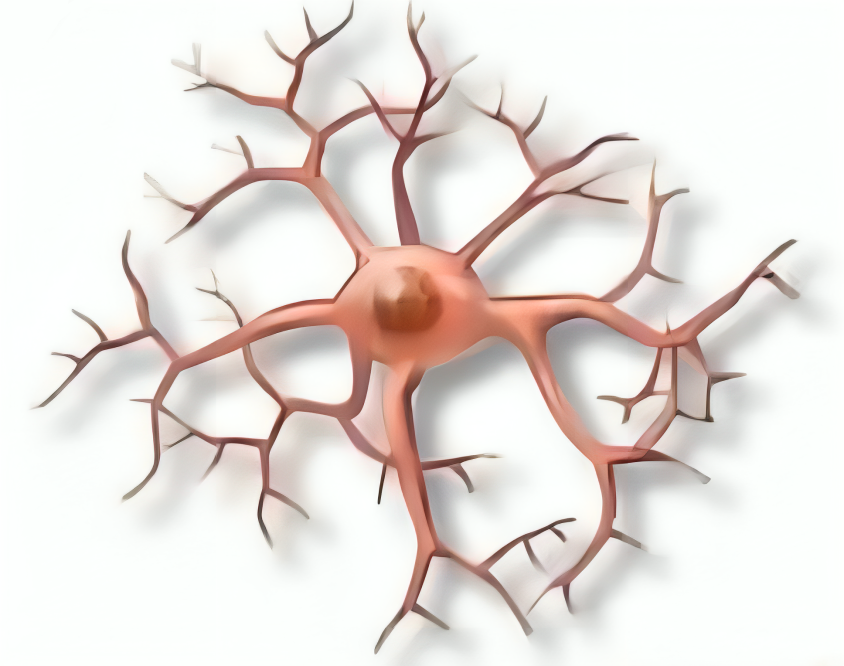
\includegraphics[width=\textwidth]{./img/microglia.png}
\end{minipage}\\[1em]

\begin{minipage}{0.79\textwidth}
    \begin{descriptionlist}
        \item[Astrocytes] \marginnote{Astrocytes}
            Star-shaped cells located in the central nervous system.
            They surround neurons and are in contact with the brain's vasculature.
            \begin{itemize}
                \item Provide nourishment to neurons.
                \item Regulate the concentration of ions and neurotransmitters in the extracellular space.
                \item Communicate with the neurons to modulate synaptic signaling.
                \item Maintain the blood-brain barrier that separates the tissues of the central nervous system and the blood.
            \end{itemize}
    \end{descriptionlist}
\end{minipage}
\begin{minipage}{0.2\textwidth}
    \centering
    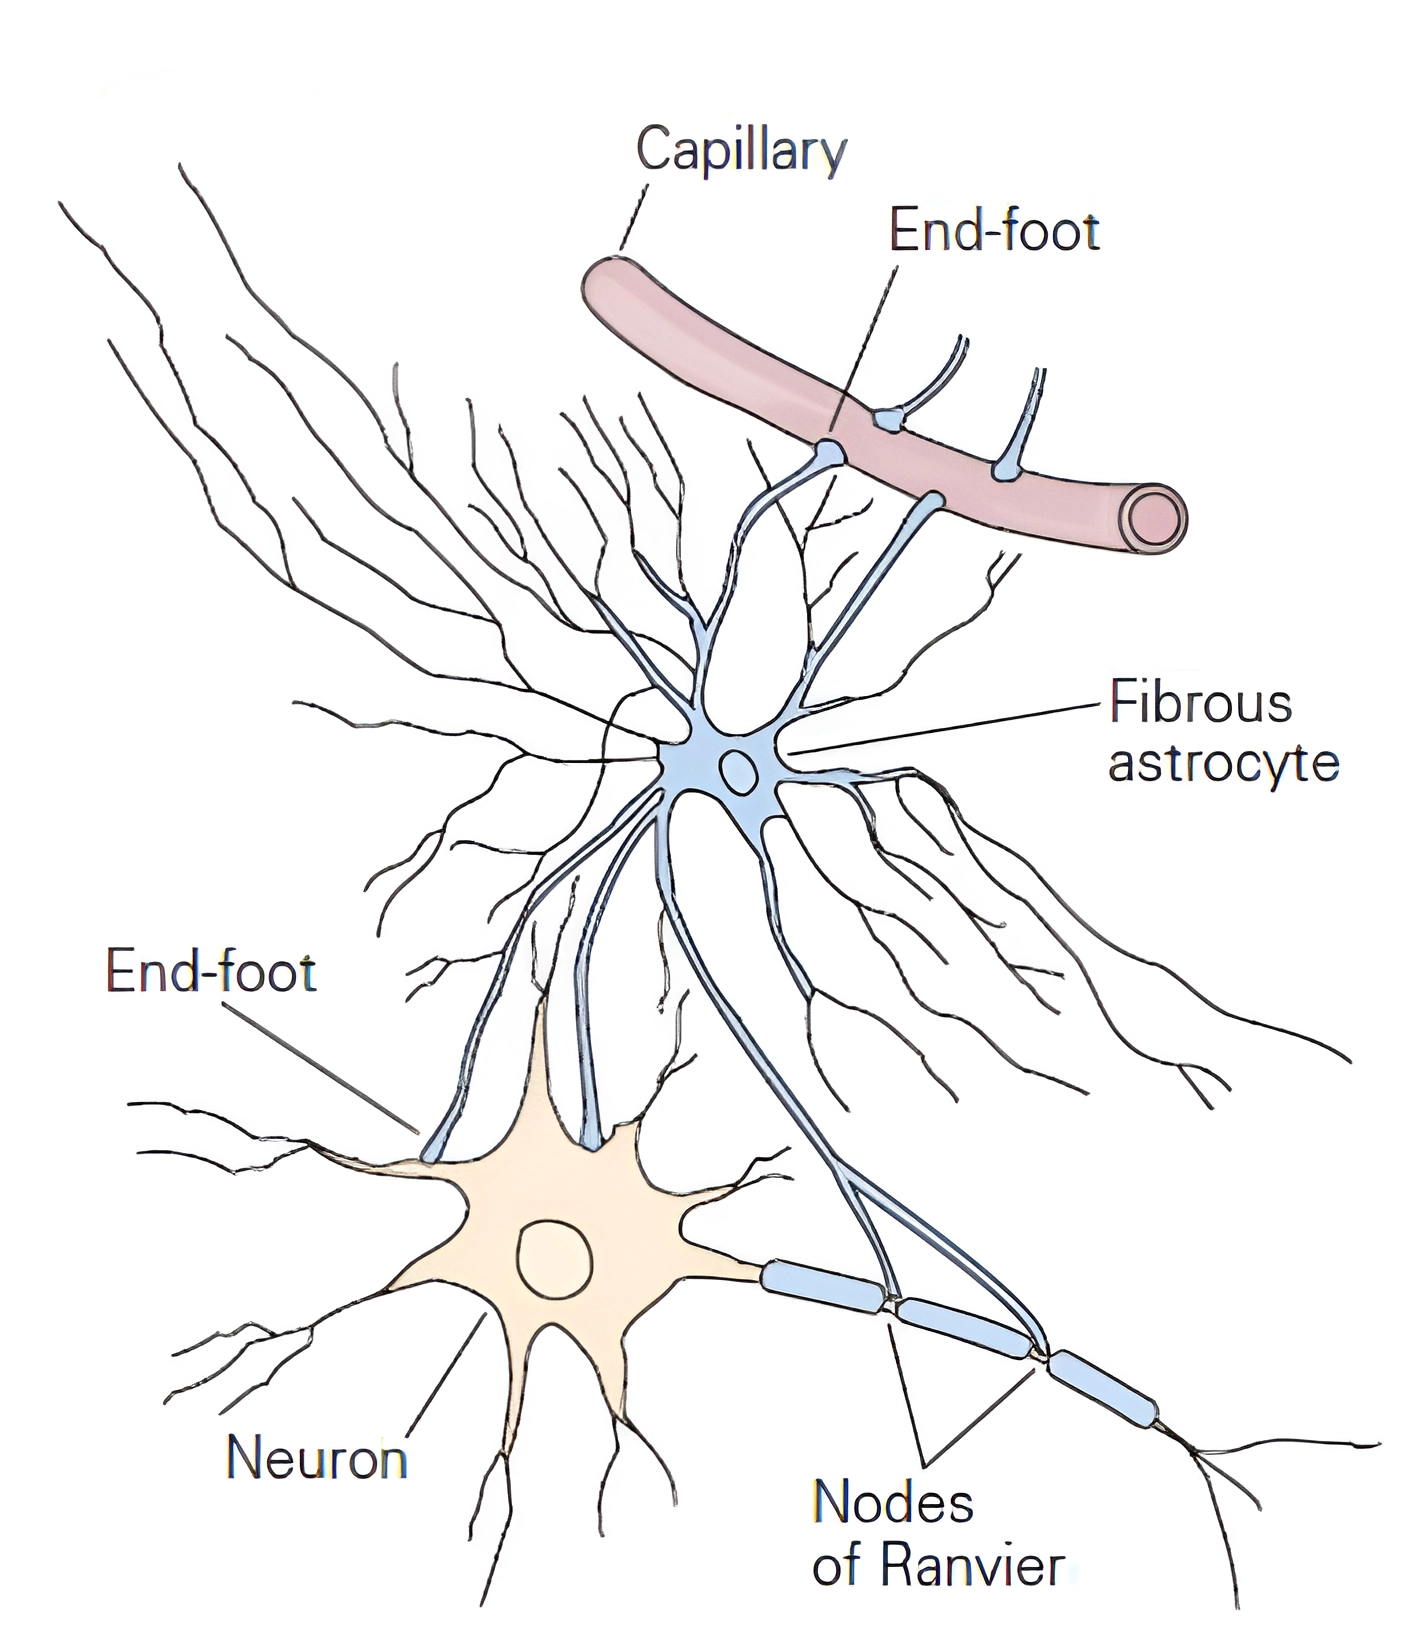
\includegraphics[width=\textwidth]{./img/astrocyte.png}
\end{minipage}\\[1em]

\begin{minipage}{0.79\textwidth}
    \begin{descriptionlist}
        \item[Oligodendrocytes and Schwann cells] \marginnote{Oligodendrocytes\\Schwann cells}
            Oligodendrocytes are located in the central nervous system, while 
            Schwann cells are located in the peripheral nervous system.
            \begin{itemize}
                \item Produce thin sheets of myelin that wrap concentrically around the axon of the neurons.
                    This insulating material allows the rapid conduction of electrical signals along the axon.
            \end{itemize}

            \begin{remark}
                Myelin is white, giving the name to the white matter.
            \end{remark}

            \begin{remark}
                In multiple sclerosis, the immune system attacks the oligodendrocytes, 
                slowing or disrupting messages traveling along the nerves.
            \end{remark}
    \end{descriptionlist}
\end{minipage}
\begin{minipage}{0.2\textwidth}
    \centering
    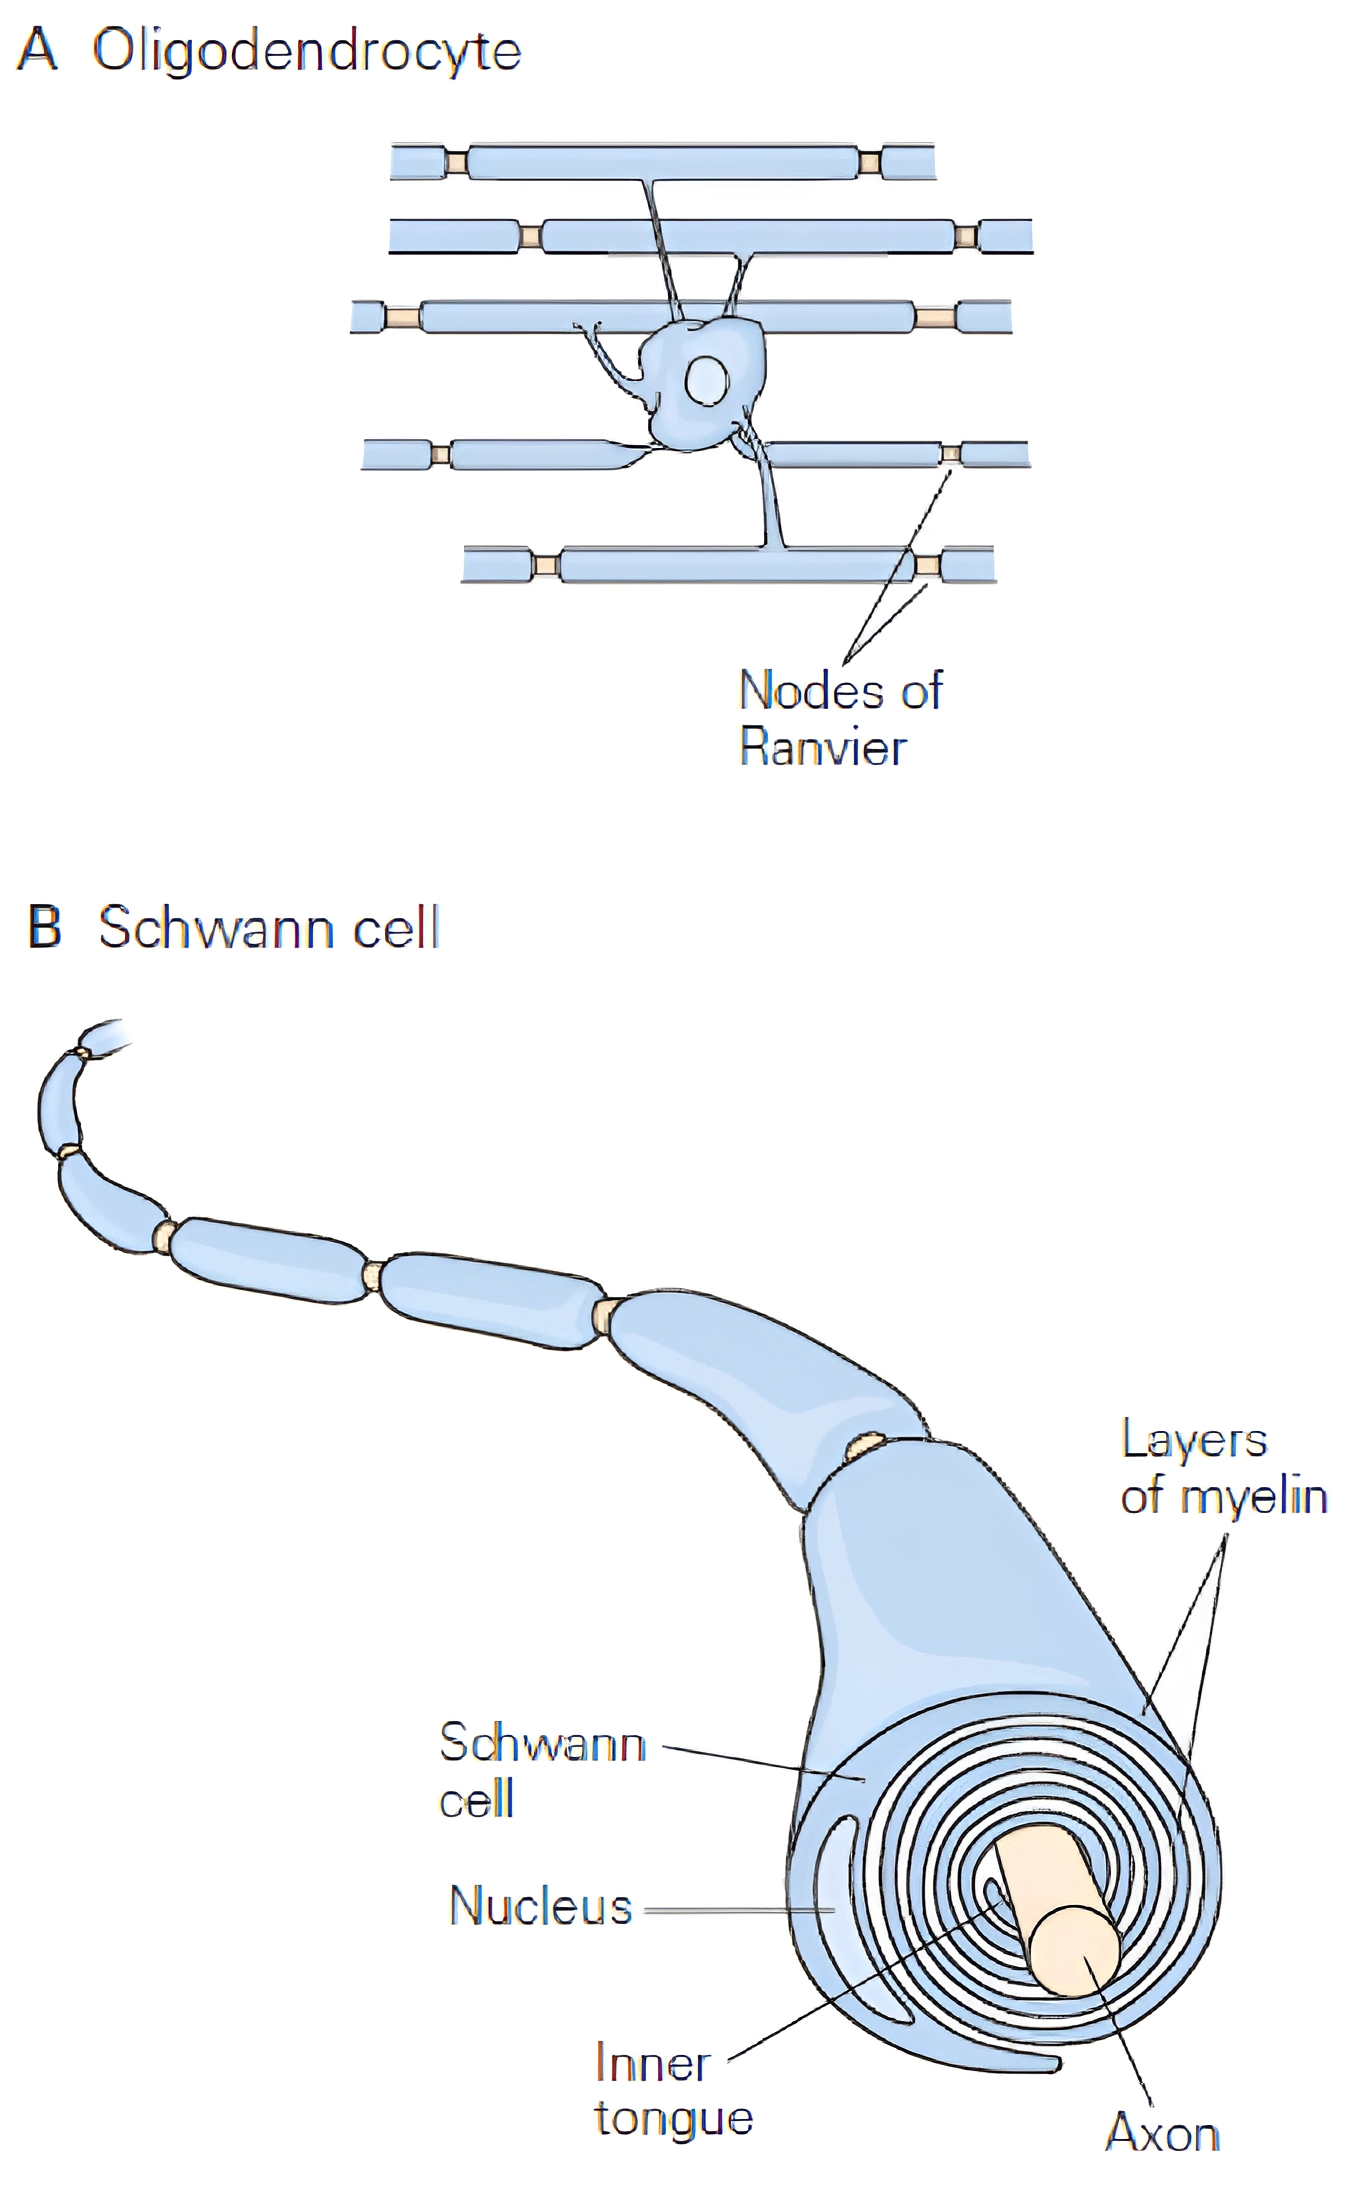
\includegraphics[width=\textwidth]{./img/insulation.png}
\end{minipage}



\subsection{Neurons / Nerve cells}
\marginnote{Neurons/Nerve cells}

A nervous system has around 100 billion neurons.
There are 100 distinct types of neurons varying in form, location, and interconnectivity.

Generally, a neuron does the following:
\begin{enumerate}
    \item Receives some information.
    \item Makes a decision.
    \item Passes it to other neurons.
\end{enumerate}

\begin{description}
    \item[Eukaryotic cell] \marginnote{Eukaryotic cell}
        A neuron is an eukaryotic cell. Therefore, it has:
        \begin{description}
            \item[Cell membrane] Membrane that separates the intracellular and extracellular space.
            \item[Cytoplasm] Intracellular fluid mainly made of proteins and ions of potassium, sodium, chloride, and calcium.
            \item[Extracellular fluid] Fluid in which the neuron sits. Similar composition of the cytoplasm.
            \item[Cell body/soma] Metabolic center of the cell.
        \end{description}

        \begin{figure}[h]
            \centering
            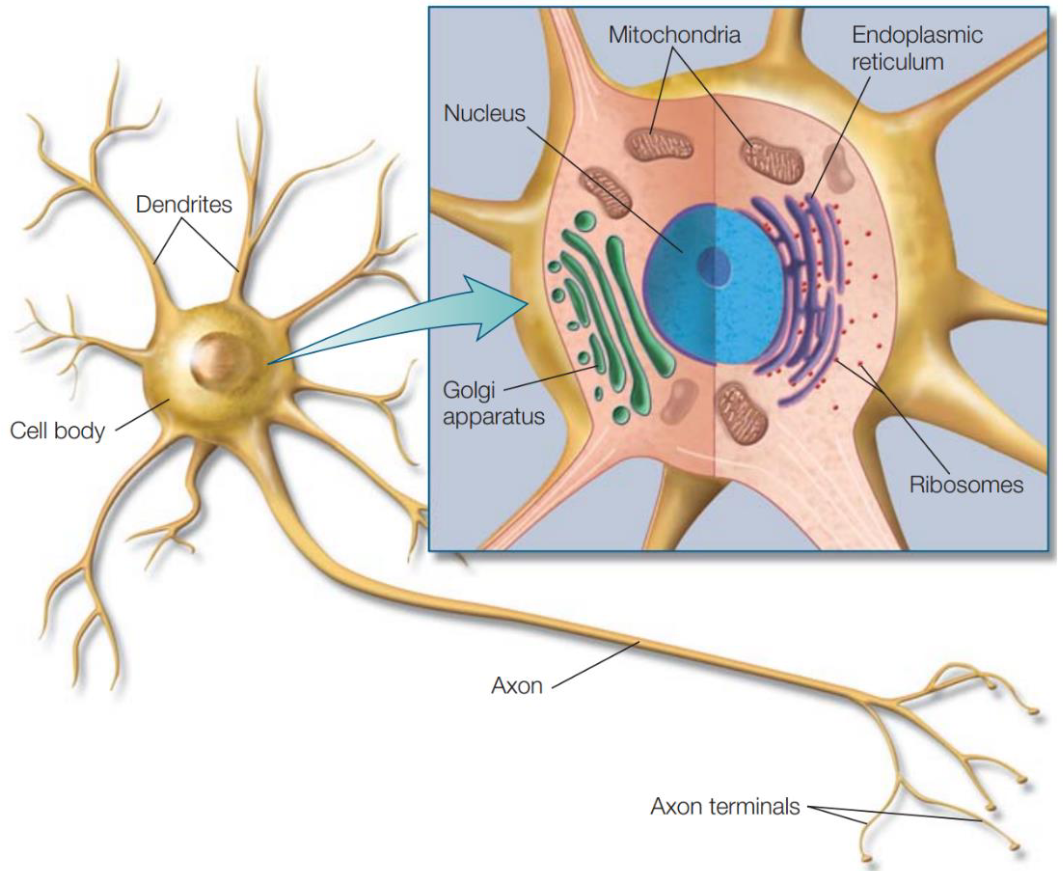
\includegraphics[width=0.5\textwidth]{img/neuron_eukaryotic.png}
            \caption{Neuron as an eukaryotic cell}
        \end{figure}
\end{description}

\begin{description}
    \item[Neuron-specific components] \phantom{}
        \begin{description}
            \item[Dendrites] \marginnote{Dendrites}
                Receives the outputs of other neurons.
                A neuron has multiple dendrites with different shapes depending on the type and location of the neuron.
            \item[Axon] \marginnote{Axon}
                Transmitting zone of the neuron that carries electrical signals from the dendrites to the synapses (from 0.1mm to 2m).
                A neuron has a single axon.
            \item[Synapses] \marginnote{Synapses}
                Represents the output zone of the neuron from where electrical or chemical signals can be transmitted to other cells.
                A neuron has multiple synapses.

                \begin{description}
                    \item[Presynaptic cell] Cell transmitting a signal.
                    \item[Postsynaptic cell] Cell receiving a signal.
                    \item[Synaptic cleft] Narrow space separating presynaptic and postsynaptic cells (i.e. the space separating two neurons).
                \end{description}
        \end{description}
\end{description}

\begin{figure}[H]
    \centering
    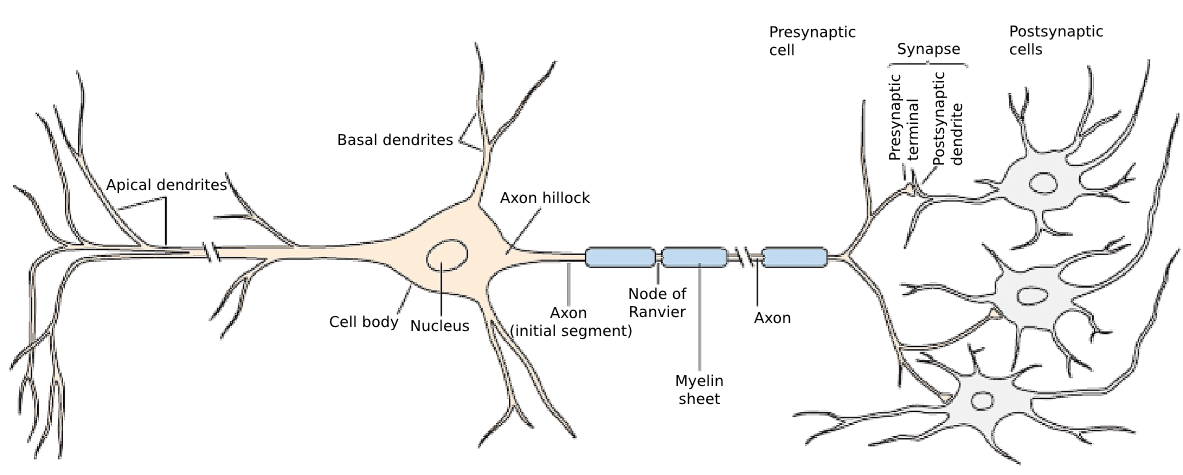
\includegraphics[width=0.9\textwidth]{img/neuron_specific.png}
    \caption{Neuron-specific components}
\end{figure}

There are three types of synapses:
\begin{descriptionlist}
    \item[Axosomatic] \marginnote{Axosomatic}
        Synapses that a neuron makes onto the cell body (soma) of another neuron.
    \item[Axodendritic] \marginnote{Axodendritic}
        Synapses that a neuron makes onto the dendrites of another neuron.
    \item[Axoaxonic] \marginnote{Axoaxonic}
        Synapses that a neuron makes onto the synapses of another neuron.
        In this case, the transmitting neuron can be seen as a signal modulator of the receiving neuron.
    \begin{figure}[h]
        \begin{subfigure}{.3\textwidth}
            \centering
            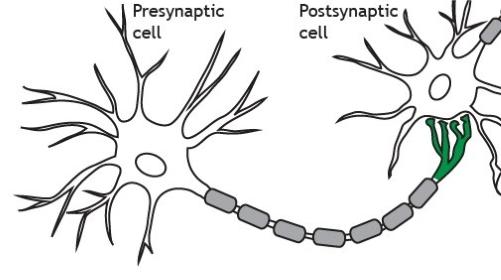
\includegraphics[width=\linewidth]{./img/axosomatic.png}
            \caption{Axosomatic}
        \end{subfigure}
        \begin{subfigure}{.3\textwidth}
            \centering
            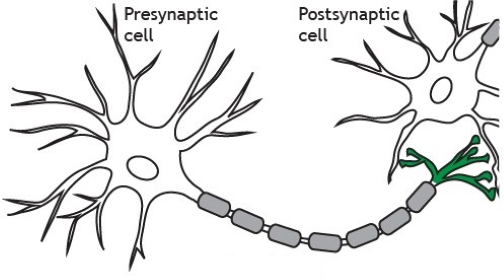
\includegraphics[width=\linewidth]{./img/axodendritic.png}
            \caption{Axodendritic}
        \end{subfigure}
        \begin{subfigure}{.3\textwidth}
            \centering
            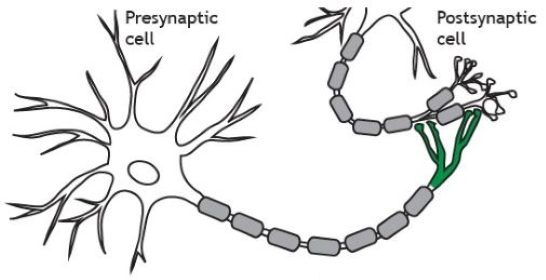
\includegraphics[width=\linewidth]{./img/axoaxonic.png}
            \caption{Axoaxonic}
        \end{subfigure}
    \end{figure}
\end{descriptionlist}

Neurons are divided into three functional categories:
\begin{descriptionlist}
    \item[Sensory neurons] \marginnote{Sensory neurons}
        Carry information from the body's peripheral sensors into the nervous system.
        Provides both perception and motor coordination.

    \item[Motor neurons] \marginnote{Motor neurons}
        Carry commands from the brain or the spinal cord to muscles and glands.

    \item[Interneurons] \marginnote{Interneurons}
        Intermediate neurons between sensory and motor neurons.
\end{descriptionlist}

\begin{description}
    \item[Principle of connectional specificity] \marginnote{Principle of connectional specificity}
        Neurons do not connect randomly but rather make specific connections at particular contact points.
\end{description}



\section{Information transfer within a neuron}


\subsection{Neuron functional regions}

In a neuron, there are four regions that handle signals:
\begin{descriptionlist}
    \item[Input zone] \marginnote{Input zone}
        Dendrites collect information from different sources
        in the form of \aclp{psp} (\acp{psp}).

    \item[Integration/trigger zone] \marginnote{Integration/trigger zone}
        \acp{psp} are summed at the axon hillock and an \ac{ap} is generated if a threshold (-55mV) has been exceeded.

    \item[Conductive zone] \marginnote{Conductive zone}
        The \ac{ap} is propagated through the axon.

    \item[Output zone] \marginnote{Output zone}
        Synapses transfer information to other cells.

        \begin{description}
            \item[Chemical synapses] The frequency of \acp{ap} determines the amount of neurotransmitters released.
            \item[Electrical synapses] The \ac{ap} is directly transmitted to the next neurons.
        \end{description}

    \begin{figure}[h]
        \centering
        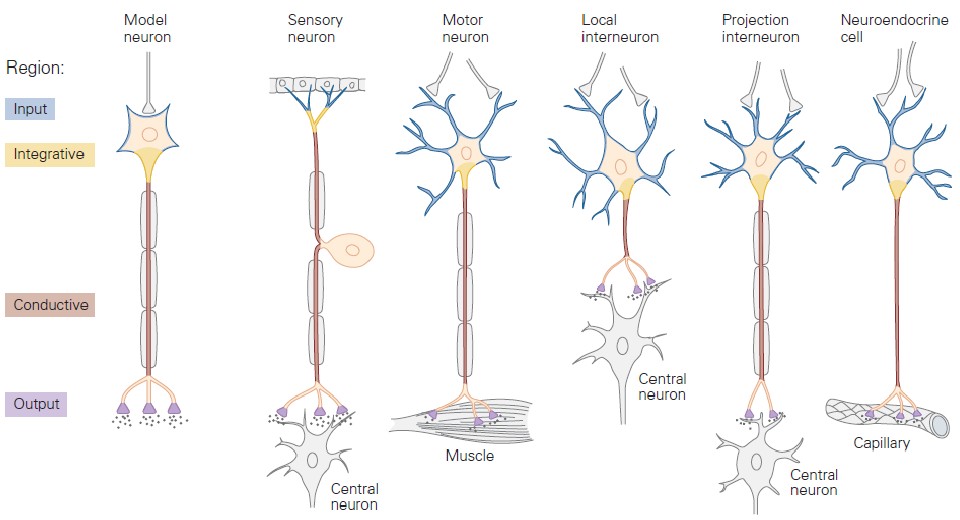
\includegraphics[width=0.8\textwidth]{./img/neuron_transmission.png}
        \caption{Transmitting regions of different types of neurons}
    \end{figure}

    \begin{figure}[h]
        \centering
        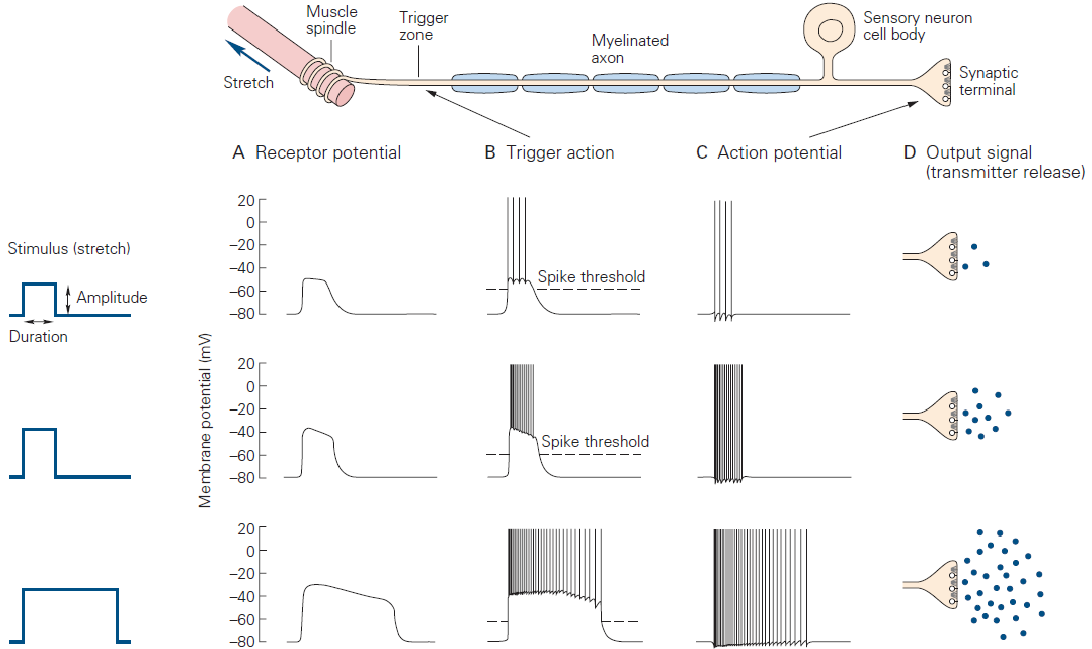
\includegraphics[width=0.8\textwidth]{./img/neuron_transmission2.png}
        \caption{Signal from the input to the output zones}
    \end{figure}
\end{descriptionlist}


\subsection{Neuron transmission signals}

\begin{description}
    \item[Resting membrane potential] \marginnote{Resting membrane potential}
        In a resting neuron, the voltage inside the cell is more negative ($-70$mV) than the outside.
        This allows the creation of an electrical signal when needed.

    \item[\Acl{psp} (\ac{psp})] \marginnote{\Acl{psp} (\ac{psp})}
        Small change in the membrane potential that alters the resting voltage of the cell.
        
        A \ac{psp} can be:
        \begin{descriptionlist}
            \item[Excitatory \ac{psp} (\acs{epsp})] \marginnote{Excitatory \ac{psp}}
                Has a depolarizing role: produces a decrease in the membrane potential (i.e. increases voltage inside the cell), 
                therefore enhancing the ability to generate an \ac{ap}.

            \item[Inhibitory \ac{psp} (\acs{ipsp})] \marginnote{Inhibitory \ac{psp}}
                Has a hyperpolarizing role: produces an increase in the membrane potential (i.e. reduces voltage inside the cell), 
                therefore reducing the ability to generate an \ac{ap}.
        \end{descriptionlist}

        A \ac{psp} has the following properties:
        \begin{itemize}
            \item The amplitude and duration of the signal are determined by the size of the stimulus that caused it.
                Overall, the amplitude is small.
            \item The signal is passively conducted through the cytoplasm, therefore it decays with distance and is able to travel 1mm at most.
            \item A single \acs{epsp} is not enough to fire a neuron. Multiple \acp{psp} are summed at the axon hillock.
                There are two types of summation:
                \begin{descriptionlist}
                    \item[Spatial summation] Sum of the \acp{psp} received at the same time.
                    \item[Temporal summation] Sum of the \acp{psp} received at different time points.
                \end{descriptionlist}

                \begin{remark}
                    The fact that a single \ac{epsp} is not enough to fire a neuron prevents a response to every single stimulus.
                \end{remark}
        \end{itemize}

    \item[\Acl{ap} (\ac{ap})] \marginnote{\Acl{ap} (\ac{ap})}
        Signal generated when the sum of \acp{epsp} exceeds a fixed threshold of $-55$mV (all-or-none).

        \begin{description}
            \item[Saltatory conduction] \marginnote{Saltatory conduction}
                Mechanism that allows a fast propagation on long distances of \acp{ap}.
                \begin{enumerate}
                    \item Depolarization causes the sodium ion (Na+) channels located in the nodes of Ranvier of the axon to gradually open.
                    \item Na+ flows into the neuron and further depolarizes it until the Na+ equilibrium potential is reached.
                    \item With Na+ equilibrium, Na+ channels close and potassium ion (K+) channels open.
                    \item K+ flows into the neuron and restores the membrane potential until the K+ equilibrium potential is reached.
                    \item With K+ equilibrium, K+ channels close and 
                        the membrane potential of the neuron is more negative than the resting potential (hyperpolarization).
                        It will gradually return to its resting potential.
                        \begin{remark}
                            During hyperpolarization, Na+ channels cannot open (refractory period).
                            This has two implications:
                            \begin{itemize}
                                \item It limits the number of times a neuron can fire in a given time.
                                \item Guarantees a unidirectional electrical current flow 
                                    (\textbf{Principle of dynamic polarization}).\marginnote{Principle of dynamic polarization} 
                            \end{itemize}
                        \end{remark}
                \end{enumerate}

                \begin{figure}[H]
                    \begin{subfigure}{.45\textwidth}
                        \centering
                        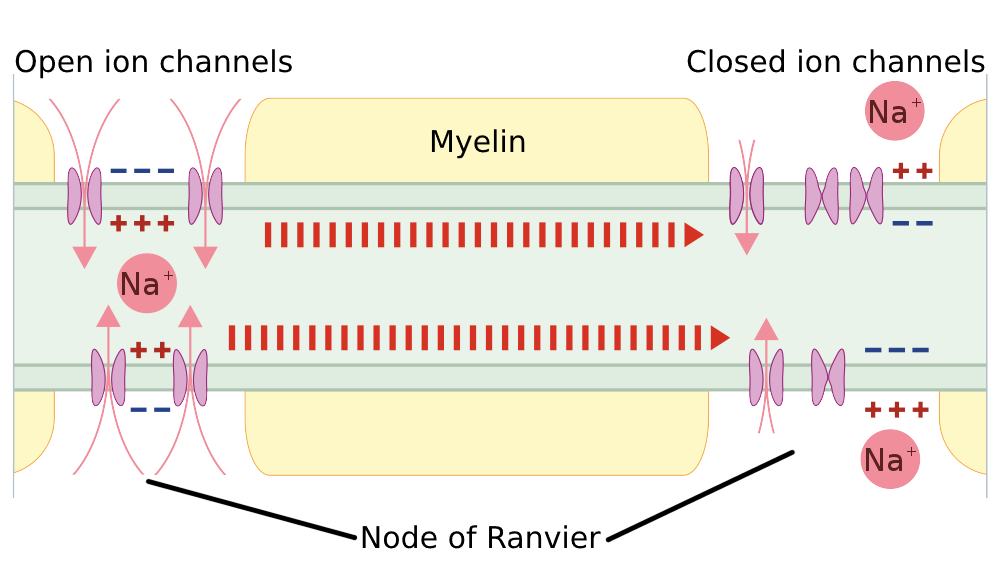
\includegraphics[width=0.85\textwidth]{./img/saltatory_conduction.png}
                        \caption{Ion channels along the axon}
                    \end{subfigure}
                    \begin{subfigure}{.45\textwidth}
                        \centering
                        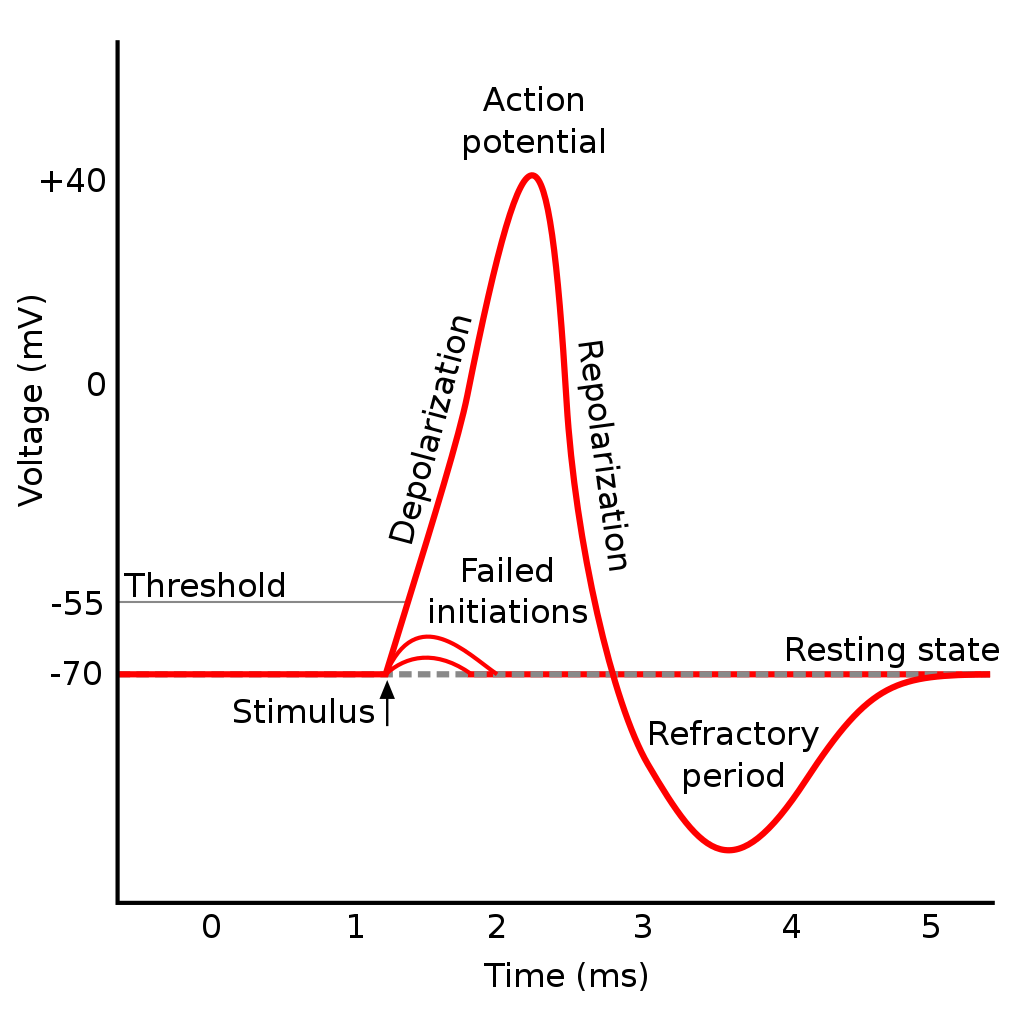
\includegraphics[width=0.8\textwidth]{./img/action_potential.png}
                        \caption{Triggering of an action potential}
                    \end{subfigure}
                \end{figure}
        \end{description}


        \begin{remark}
            As the signal is constantly regenerated, 
            \Acp{ap} have similar amplitude and duration in all neurons, regardless of the characteristics of the input \acp{psp}.
            Therefore, the only way an \ac{ap} has to carry information is by varying frequency and firing duration, making it a binary signal.
        \end{remark}
\end{description}

\begin{example}
    Seizures are caused by misfiring neurons.
\end{example}